
\section*{Cíle laboratoře}
\begin{itemize}
  \item Seznámení se signalizačním protokolem SIP.
  \item Peer-to-peer VoIP pomocí signalizace SIP.
  \item Komunikace VoIP pomocí signalizace SIP přes ústřednu.
\end{itemize}

\section*{Základní instrukce}
\begin{itemize}
  \item Připojte k počítači headset se sluchátky a mikrofonem.
  \item Přihlaste se do CentOS (F3), user/password {\tt user}/{\tt user4lab}.
  \item V pravé horní části obrazovky {\bf zkontrolujte nastavení zvuku}. Sluchátka a mikrofon nastavte na optimální hlasitost.
  \item Otevřete si příkazovou řádku pro uživatele {\tt user}.
  \item Otevřete si příkazovou řádku pro uživatele {\tt root} příkazem {\tt su} (switch user).
  \item V případě potřeby si otevřete další terminál v novém okně.
  \item Pro editaci konfiguračních souborů použijte libovolný editor (např. nano, vim, gedit).
  \item Pracujte ve dvojicích, zkontrolujte, že máte počítač propojen
    přímým kabelem s přístupovým přepínačem (rozhraní enp2s0, zdířka E na patch panelu).
\end{itemize}

\section*{Úkoly}
\section{Peer-to-peer VoIP pomocí signalizace SIP}
Se svým sousedem nastavte komunikaci VoIP mezi Vašimi dvěma počítači bez použití ústředny (spojení peer-to-peer).

\begin{enumerate}
    \item Zapněte program Ekiga Softphone a vyčkejte až se spustí okno programu.
    \item V menu {\bf Options} $\rightarrow$ {\bf Preferences} $\rightarrow$ {\bf Manage SIP accounts} nastavte pole Your username na hodnotu {\bf 10XX}, kde {\bf XX je číslo Vašeho počítače}.
    \item Spusťte síťový analyzátor Wireshark a začněte zachytávat pakety na rozhraní, kterým jste připojeni k síti.
    \item Po spuštění nastavte filtr tak, aby zobrazoval pouze protokol SIP (Filter: sip).
    \item V hlavním okně programu zadejte do spodního pole SIP adresu Vašeho souseda: {\bf sip:10.10.10.1YY}, kde {\bf YY} je číslo počítače Vašeho souseda.
    \item Zavolejte Vašemu sousedovi stisknutím zeleného telefonu. Na druhém počítači přijměte hovor, vyzkoušejte, zda se se sousedem navzájem slyšíte a po chvíli hovor ukončete.
(V případě problémů se zvukem zkontrolujte, zda není v systému ztlumen mikrofon, či audio výstup, případně v aplikaci Ekiga Softphone v menu Edit $\rightarrow$ Preferences $\rightarrow$ Audio $\rightarrow$ Devices zkontrolujte nastavení zvukových zařízení.) 
    \item Proveďte analýzu navazování spojení v odchycených datech ve Wiresharku. Využijte podpory v menu {\bf Telephony $\rightarrow$ VoIP Calls}, kde uvidíte jednotlivé zaznamenané hovory. Vyberte příslušný hovor a pro zobrazení průběhu klikněte na volbu {\bf Flow}.
    \item Zakreslete spojení do grafu v protokolu. Uveďte, pomocí kterých protokolů a mezi jakými IP adresami a porty probíhá signalizace a přenos dat. Zjistěte použitý kodek pro přenos hlasu.
\end{enumerate}
Názvy a čísla podporovaných kodeků lze zobrazit v SIP/SDP zprávě v sekci {\bf Session Initiation Protocol} $\rightarrow$ {\bf Message body} $\rightarrow$ {\bf Session description protocol}:
\begin{figure}[h!]
  \centering
  \fbox{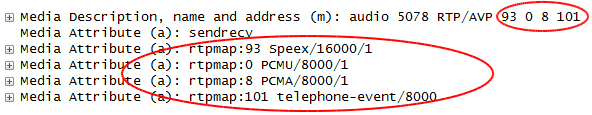
\includegraphics[width=145mm]{img/3a.png}}
\end{figure}

\noindent Informace o tom, který z podporovaných kodeků byl skutečně použit získáte z RTP paketů (Filter: RTP) podle čísla v poli {\bf Payload type}.
\begin{figure}[h!]
  \centering
  \fbox{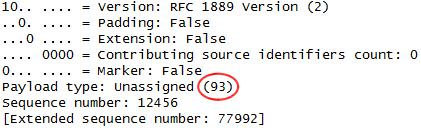
\includegraphics[width=105mm]{img/3b.png}}
\end{figure}


\section{Komunikace VoIP pomocí signalizace SIP přes ústřednu}
Se svým sousedem nastavte komunikaci VoIP mezi vašimi dvěma počítači pomocí SIP ústředny vašeho ISP.

\subsection{Analýza registrace a odregistrace}
\begin{enumerate}
    \item Spusťte znovu zachytávání paketů v aplikaci Wireshark tlačítkem 
\includegraphics[width=3mm]{img/ws_start.png}.
    \item Vraťte se do hlavního okna aplikace Ekiga Softphone, otevřite menu {\bf Edit} $\rightarrow$ {\bf Accounts}.
    \item V otevřeném okně použijte menu {\bf Accounts} $\rightarrow$ {\bf Add a SIP Account} a zobrazené formuláři vyplňte: \\
    ~\\
    {\bf Name:} {\tt <Vaše jméno>}
    {\bf Registrar:}{\tt 10.10.10.222} \\
    {\bf User:} 	{\tt userXX} \\
    {\bf Authentication user:} 	{\tt <nechte prázdné>} \\
    {\bf Password:}	{\tt hesloXX} \\
    {\bf Timeout:} {\tt 3600}
    ~\\
    a potvrďte tlačítkem {\bf OK}.
    \item Tímto jste provedli registraci k ústředně. Pokud jste vše nastavili správně, mělo by se ve sloupci {\bf Status} zobrazit {\bf Registred} \\
    {\it (V případě neúspěchu v nastavení účet odeberte a znovu přidejte. Pokud ani toto nepomohlo, ukončene Ekiga Softphone, spusťte /root/isa4/clean.sh a postupujte znovu od kroku 1)}
    \item V menu {\bf Edit} $\rightarrow$ {\bf Accounts} vytvořený SIP účet a klikněte na {\bf Remove}, čímž by měla proběhnout odregistrace od ústředny.
    \item Ve Wiresharku analyzujte registraci a odregistraci a zakresleslete jejich průběh do protokolu. Vyplňte požadované údaje a zjistěte, v čem se liší paket, kterým se registrujete, od paketu, kterým se odregistrujete.
\end{enumerate}


\subsection{Analýza hovoru přes ústřednu}
\begin{enumerate}
    \item Znovu se registrujte k ústředně.
    \item Obnovte zachytávání paketů v aplikaci Wireshark tlačítkem  
\includegraphics[width=3mm]{img/ws_start.png}.
    \item V hlavním okně programu zadejte do spodního pole SIP adresu Vašeho souseda: {\bf sip:10YY@10.10.10.222}, kde YY je opět číslo počítače Vašeho souseda.
    \item Zavolejte Vašemu sousedovi a proveďte analýzu hovoru podobně jako u Peer-to-peer hovoru.
    \item Zakreslete průběh spojení do grafu v protokolu. Uveďte, mezi kterými IP adresami a porty probíhá signalizace a mezi kterými přenos dat. Vyplňte, které protokoly se používají pro signalizaci a které pro přenos. Dále zjistěte, jaký kodek pro přenos hlasu byl použit.
\end{enumerate}

\section{Ukončení práce v laboratoři}
\begin{itemize}
  \item Počítač vypněte spuštěním (jako {\bf root}) skriptu {\tt /root/isa4/clean}.
\end{itemize}
